\documentclass[12pt,a4paper,twosided]{article}

% Compile with "pandoc -S --template=design.template.tex design.md -o design.tex"
% Then add a:
% 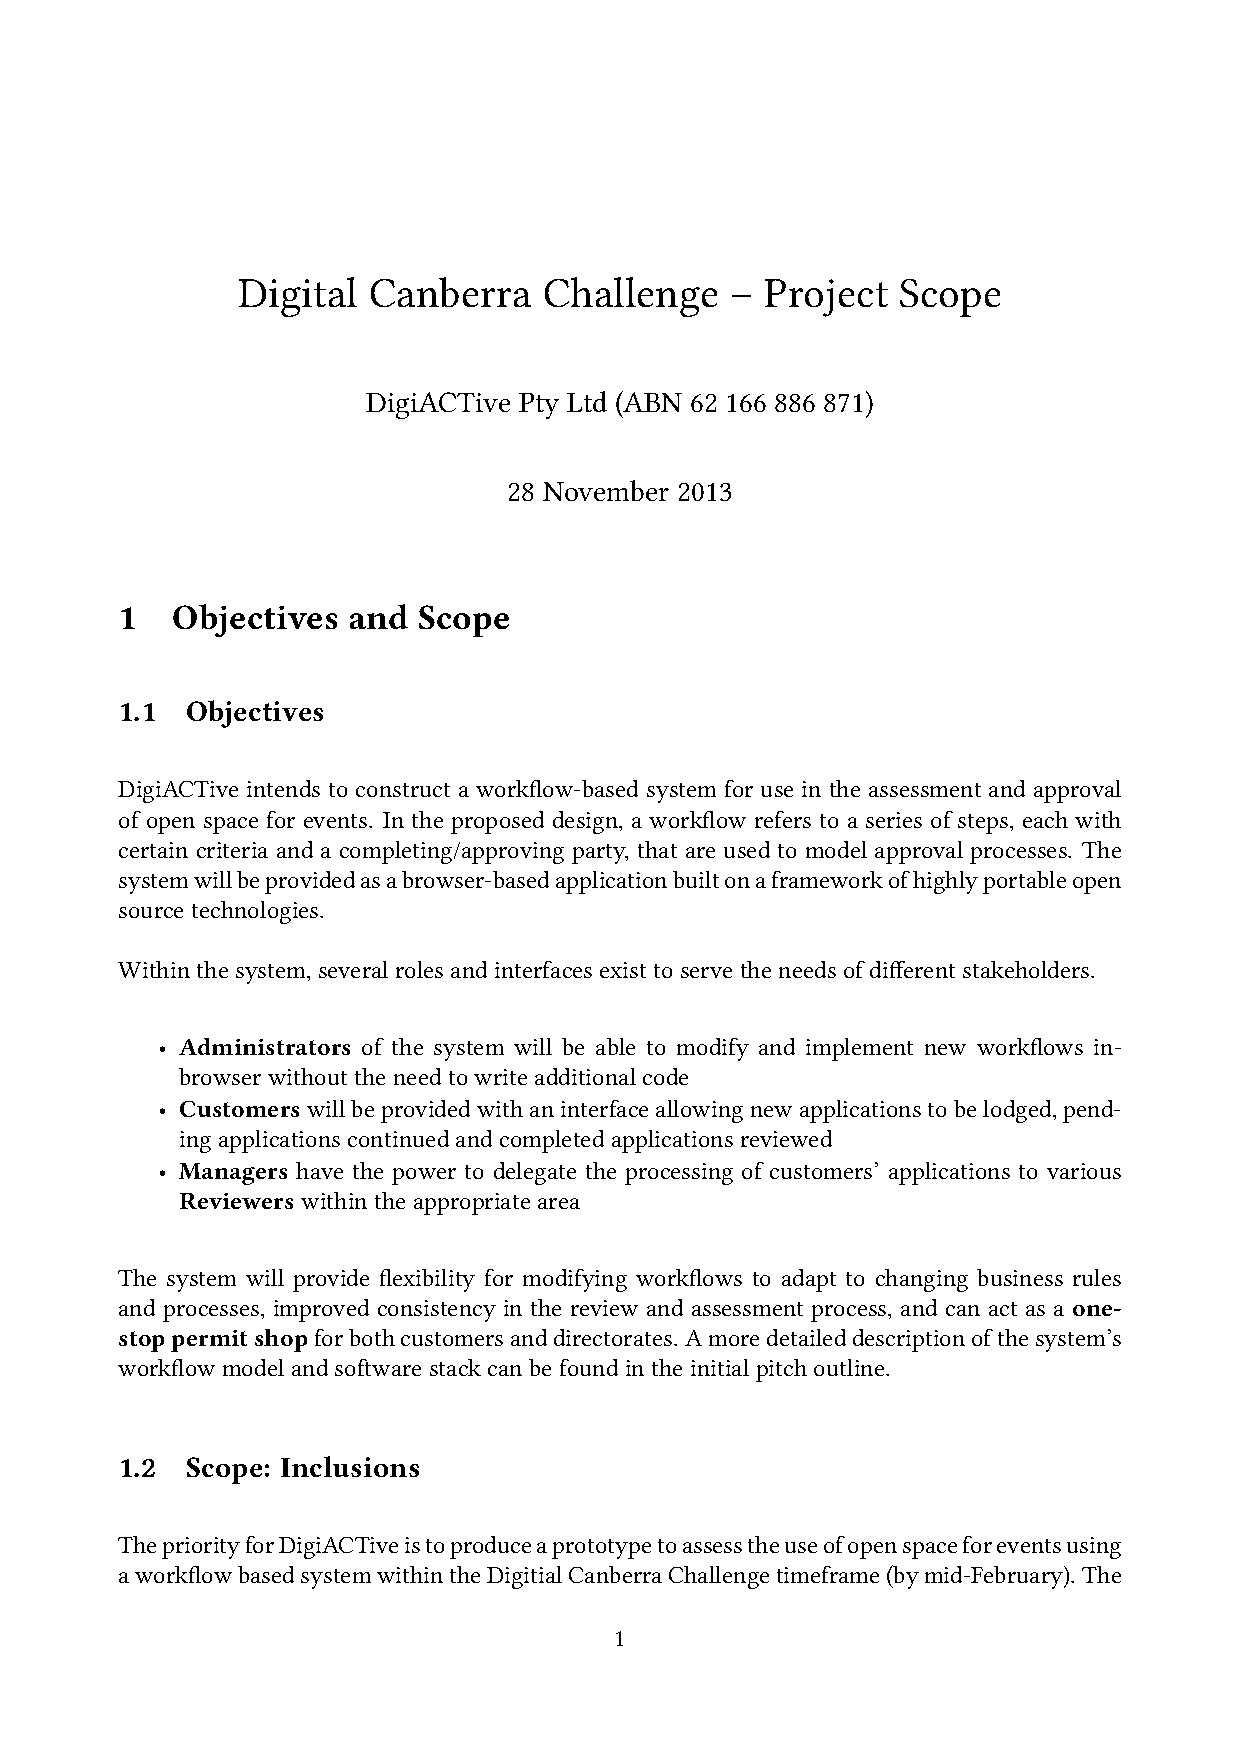
\includepdf[pages=1-6,nup=1x2,frame=true,landscape=true]{attached_work_scope.pdf}
% point, and remove the ?raw=true from the graphics, and add [width=0.9\textwidth]


\usepackage[utf8]{inputenc}
\usepackage{amsmath}
\usepackage{amsfonts}
\usepackage{amssymb}
\usepackage[top=3cm,bottom=3cm,left=2cm,right=2cm]{geometry}
\usepackage{framed}
\usepackage{setspace}
\setlength{\parindent}{0.0in}
\setlength{\parskip}{0.2in}
\usepackage{longtable}
\usepackage{float}


%\usepackage{times}
%\usepackage[T1]{fontenc}
%\usepackage{libertine}
\usepackage{graphicx}
\usepackage{pdfpages}
\usepackage[colorlinks=true, urlcolor=blue]{hyperref}
\renewcommand*\oldstylenums[1]{{\fontfamily{fxlj}\selectfont #1}}
\title{Digital Canberra Challenge: Round 1 - Case Study}
\author{DigiACTive Pty Ltd}
\date{March 2014}
\begin{document}
\maketitle
\newpage
\section{Executive Summary}

DigiACTive Pty Ltd set out to provide Canberrans with a simpler, more
efficient way to get the various approvals required to run events.
Through the Digital Canberra Challenge, with the involvement of Parks and
City Services in TAMS, and the eGov Cluster in NICTA, we scoped,
designed and built a proof of concept system over the summer of
2013-2014.

Our solution provides a one-stop shop for approvals, based on the
concept of ``workflows''. Workflows are defined as a set of steps with a
desired outcome. Workflow steps can collect information from clients by
requiring them to fill out a form, answer questions, or upload a
document. Steps can also require action from staff at the approving
directorate, such as reviewing and verifying client information.
Workflows can be built in the system with a point-and-click editor.

Our solution addresses a number of citizen concerns:

\begin{itemize}

\item
  It provides a single point of contact for an application, so clients
  can ask questions and resolve issues along the way.
\item
  It provides a consolidated communications register, so all
  communication is in one place.
\item
  It keeps clients up to date on the progress of their application, and
  provides increased visibility into its progress.
\item
  It keeps a record of past applications, to reduce the workload when
  similar events are run repeatedly.
\item
  For events that require approval from a number of directorates, it
  provides simple integration of those workflows, without requiring the
  client to enter the same information over and over again.
\end{itemize}

Our solution also increases directorate efficiency, and increases
management visibility into staff workloads and performance.

We believe our solution could be made production ready and deployed. It
is sustainable, scalable, and in line with the Digital City Action Plan
and the Strategic Plan for ICT 2011-2015.

\newpage
\section{Description of challenge}

A thriving, vibrant city should make it easy for citizens and small
businesses to run public events. At the same time, regulations and
permit systems are needed to make sure that events are run in a safe,
community-friendly and sustainable way.

Unfortunately, the proliferation of regulations and permits has made
running events into something more akin to navigating a maze. We set out
to provide Canberrans with a simple, efficient way to navigate that
maze.

\subsection{Our solution: a birds-eye view}

Our proof-of-concept demonstrates a system that:

\begin{itemize}

\item
  provides residents and businesses with a clear, streamlined way to
  work through the various approvals they require.
\item
  provides a central point of contact so that, as far as possible, a
  single public servant sees the process through from start to finish
  and is able to help resolve problems as they come up.
\item
  lays out the requirements clearly, helping directorates to ensure that
  applicants understand what is required of them and can meet those
  requirements with a minimum of fuss.
\end{itemize}

Our solution is browser-based application built on the concept of
modelling approval processes as \textbf{workflows}. A workflow is a
series of steps with a desired end point. Each step contains certain
actions that need to be completed, either by a client or by directorate
staff.

\begin{framed}
For example, a workflow could be:

\begin{itemize}

\item
  Apply to use public unleased land
\item
  Apply for a liquor license
\item
  Apply for a fireworks display permit
\end{itemize}

Workflow steps could include:

\begin{itemize}

\item
  ``Enter event details''. Completed by a customer, by filling out an
  online form. The step would lay out what questions are mandatory and
  which are optional, and provide tips and a way to ask for advice.
\item
  ``Preliminary risk assessment''. Completed by a customer, by filling out an online form. The step would ask a number of questions about the event's risk factors, and automatically apply business rules to determine whether a risk management plan is necessary.
\item
  ``Upload a risk management plan''. Completed by a customer, by
  uploading a document. The step lays out the requirements for a risk
  management plan, and provides a link to a template and the information
  that the document must include.
\item
  ``Review risk management plan''. Completed by an approver within a
  directorate, after reviewing a risk assessment plan. The step lays out
  the internal procedures for assessing these documents, so that there
  is consistency within the Directorate.
\item
  ``Issue permit''. Completed by an approver within a directorate, after reviewing the entire application. The step allows the approver to create or upload a permit document that is consistent with legislative and administrative requirements.
\end{itemize}
\end{framed}

The system has been designed around the needs of regular citizens,
community groups, businesses and Directorates:

\begin{itemize}

\item
  Citizens are provided with an interface allowing new applications to
  be lodged, pending applications continued and completed applications
  reviewed.
\item
  Community groups and businesses are provided with powerful tools to
  maintain the integrity of their accounts and data as their membership
  changes.
\item
  Within directorates:
\begin{itemize}
\item
  Approvers are tasked with reviewing applications.
\item
  Delegators manage the workload of approvers, delegating the processing
  of customers' applications to various approvers within their area.
\item
  Administrators are able to modify existing workflows and implement new
  workflows in a point and click manner.
\end{itemize}
\end{itemize}

The system provides flexibility for modifying workflows to adapt to
changing business rules and processes, improving consistency in the
review and assessment process. The system can act as a \textbf{one-stop
shop} for permit applications for both customers and directorates.

\subsection{Key Details}


\begin{table}[h!]
  \centering
  \begin{tabular}{|c|l|}
    \hline
Competition & \href{http://digitalcanberrachallenge.com.au}{Digital Canberra Challenge} Round 1 \\ \hline
Challenge & \textbf{Quicker event approvals}: Improve the process for gaining permits for music \& other cultural events in the ACT. \\ \hline
Involved Parties & DigiACTive Pty Ltd, eGov Cluster (NICTA), ACT
Government \\ \hline
ACT Government Involvement & Parks and City Services, TAMS \\ \hline
Timeframe & 1 November 2013 - 17 March 2014 \\ \hline
Budget & \$5000 for reimbursement of expenses \\ \hline
Deliverables & Proof of Concept System, this Case Study \\ \hline
Contacts & DigiACTive: Daniel Axtens at
\href{mailto:daniel@axtens.net}{\href{mailto:daniel@axtens.net}{daniel@axtens.net}} \\ \hline
  \end{tabular}
  \caption{Key Details}
  \label{tab:keydetails}
\end{table}

Due to the limited time-frame of the competition, the scope of the project was restricted to a proof-of-concept system, rather than a fully functional, deployable system.


\newpage
\section{Methodology}

DigiACTive tackled the challenge over the 2013-14 summer.

\subsection{Forming the team and the concept}

We first became aware of the challenge as individuals in late 2013. The
challenge was discussed informally amongst the ANU Computer Science
Students' Association, and from that a team of three undergraduate ANU students was formed.

We initially approached the technical side of things in general terms:

\begin{itemize}

\item
  We firstly settled on the idea of a workflow engine, after briefly
  toying with an enhanced Smart Forms system and a Finite State Machine
  solution.
\item
  Because we had existing expertise in development in the team, we built
  an open source stack around technologies we already knew and
  trusted.
\item
  Due to the short time frame of the competition, we verified that the
  bulk of the project could be built by composing existing open source
  components.
\end{itemize}

Once we satisfied ourselves that we could deliver, we proceeded to pitch
our concept.

\subsection{Pitching the team's solution}

The requirement to write a formal pitch was helpful in forcing us to do
a more formal sort of design that we might otherwise have done. We had
to consider scalability (although we perhaps understood it in a
different, more technical, way to what the was expected) and
sustainability, which lead us to do more careful design and planning.
This up-front design stood us in good stead for implementation.

Having submitted the written pitch, we were somewhat surprised to be
called in to do an in-person pitch, especially when we realised the sort
of competition that we were up against. However, we found the process to
be helpful in refining our understanding of the problem and the needs
our solution was trying to meet.

\subsection{Bake-off}

We were selected as one of two teams to proceed to implement a
proof-of-concept.

The process of building our solution then fell into a
number of phases:

\begin{itemize}

\item
  Formalise the team structure and sign the necessary agreements.
\item
  Formally plan the project, including scope and design documents.
\item
  Build ``Milestone 1'': a prototype that ran a predefined static
  workflow.
\item
  Test Milestone 1.
\item
  Build ``Milestone 2'': an extension of the Milestone 1 prototype that
  supported dynamically editing workflows.
\end{itemize}

The process was facilitated by the eGov Cluster at NICTA, who did an
admirable job and made the administrative side much more manageable.

\subsubsection{Formalising the team}

We turned our unnamed team into DigiACTive Pty Ltd, signed the
necessary project agreements and purchased the necessary insurance
cover. This was a surprisingly challenging, time-consuming and expensive
process.

\subsubsection{Requirements Definition}

We conducted a process of consultation with various stakeholders involved
in events organisation to further refine the requirements our system should 
meet. These stakeholders included:

\begin{itemize}

\item
  The event coordinator of a major territory community festival.
\item
  Representatives from MusicACT: an organisation with regular exposure 
  to event planning in the territory and responsible for proposing 
  this problem for the inaugural Digital Canberra Challenge.
\item
  Parks and City Services (TAMS): The directorate responsible for
  administering the current public unleased land approval process and the
  potential future administrators of our proposed system.
\end{itemize}

\subsubsection{Scope}

Nailing down the precise scope of the challenge also proved to be more
involved than we expected, as we attempted to simultaneously include a
reasonably large feature set while making sure we could finish what we
started within the timeframe. Ultimately a scope document was prepared
and signed off on, which kept our scope manageable.

Throughout the process, there were a number of items that came up that
would be within the scope of a fully deployed system, but which we did
not want to commit to for the prototype. These items were collated into
a Considerations Register administered by NICTA. This proved to be an
excellent way of dealing with these considerations -- they are now on
record should we proceed to implement a production system, without them
causing scope creep while working on the prototype.

\subsubsection{Milestones}

Having defined the scope, we created a formal project plan, which split
the project into two major milestones.

\begin{itemize}

\item
  Milestone 1: a prototype that ran a predefined static workflow
\item
  Milestone 2: an extension of the Milestone 1 prototype which supported
  the dynamic editing of workflows.
\end{itemize}

The system that we built is described in detail in Section~\ref{sec:solution}. 

As far as the
process of building goes, we found that, for technical reasons,
Milestone 1 was more time-consuming than we expected, but Milestone 2
was slightly less time-consuming.

\subsubsection{Project wind-up}

Following a successful demonstration of Milestone 2 to TAMS, the team
shifted to winding up the Digital Canberra Challenge competition
requirements - preparing presentations, the source code, documentation,
and this case study.

We have also been investigating how to take the project further after
the close of the competition.

\subsubsection{Project governance}

Throughout the project, we had fortnightly meetings with the project
board, consisting of a representative from DigiACTive, a representative
from TAMS, and a representative from the eGov Cluster at NICTA.

These meetings were incredibly valuable for keeping us on track and
accountable for the progress we were making. We'd like to acknowledge
the excellent work of Rachel Reid, who represented TAMS, and Michael
Phillips who represented NICTA, as well as the vital administrative
support of NICTA's Ana Belgun.

\newpage
\section{Proposed solution}
\label{sec:solution}
\subsection{The prototype in overview}

\subsubsection{The core: Workflow Engine}

At the core of the solution is a ``workflow engine''.

The system is premised on the observation that most permit applications can be broken down into a number of interrelated steps, with well understood linkages between the steps. Some steps are taken by the customer, and some steps are taken by the approving agency. For example, a sample workflow is shown below in Figure~\ref{fig:sample-workflow}. Here, steps in blue are taken by the customer, and steps in green are taken by the approving agency.

\begin{figure}[h!]
  \centering
  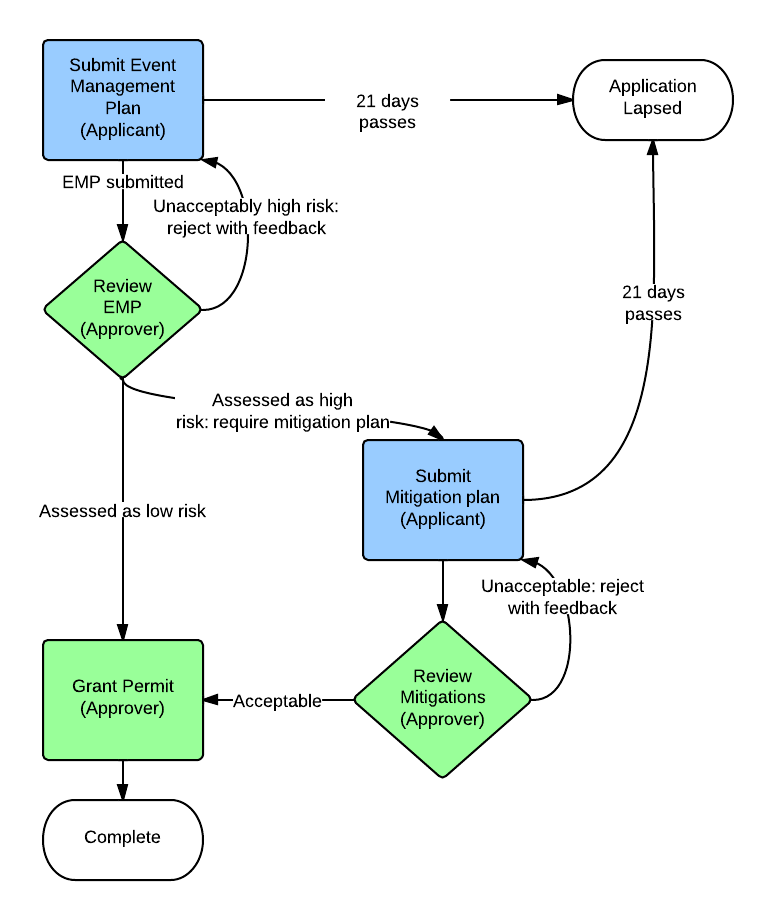
\includegraphics[width=0.6\textwidth]{sample-workflow.png}  
  \caption{A sample workflow.}
  \label{fig:sample-workflow}
\end{figure}

Notably, a workflow allows more flexible processes than a single, linear application. As shown in the sample workflow, steps can happen in parallel, certain steps can be repeated, and so on.

\paragraph{What can the steps contain?}

Steps are designed to be flexible, and cover as broad a range of different scenarios as possible.

Steps can include:
\begin{itemize}
\item Filling out a form. Questions can be:
  \begin{itemize}
  \item Optional or mandatory.
  \item Free text or check boxes. Both exclusive choice (either A or B or C) and multiple choice (any combination of A or B or C) are supported. 
  \end{itemize}

  In addition, check boxes can be used to determine the steps in the workflow:
  \begin{itemize}
  \item A step can ask whether alcohol will be served at an event, and if so, the applicant will be directed to a liquor licence permit.
  \item A step can do a points-based assessment. For example, various hazards may be worth different numbers of points, and if a points threshold is reached, different risk assessment procedures can be applied.
  \end{itemize}
\item Uploading a document, for example, a risk assessment and management plan, or a permit.
\item Accepting an agreement, for example an Acceptable Use Agreement, or Permit Terms and Conditions.
\end{itemize}

Steps can have descriptive text attached to them. For example, a step which requires someone to upload a risk assessment can provide information about how to do a proper risk assessment, and a link to a template. Information can also be provided on steps done by approvers, to enhance the consistency of the approvals process.

\paragraph{How are multiple agencies handled?}

A major pain point for customers is dealing with multiple agencies: for example, when running an event, needing to deal with TAMS, JACS, AFP, and so on. It is often unclear when permits are required from these agencies and when they are not. Furthermore, each agency needs some of the same information, and some different information. 

The system has a multi-pronged approach to reducing the confusion inherent in multiple-agency applications.
\begin{itemize}
\item The system supports embedding workflows within other workflows. For example, if the workflow for the use of public unleased land determines that a liquor license is required, the system can embed the liquor license workflow. The liquor license workflow is still managed by the relevant directorate, not by TAMS, so there's no duplication of effort.
\item Embedded workflows can also be used to allow multiple-agency sign-off on a single approval decision. For example, many public unleased land applications must be approved by the ACT Insurance Authority. The system can automatically send the workflow to relevant ACTIA approvers, reducing the need for TAMS officials to manually inform other agencies.
\item Information can be shared between related workflows by ``tagging'' common questions. For example, an event's date is common across all the permit applications, so every question that asks for the event date will be tagged with a common, descriptive tag. Then, if a step encounters a tagged question that has been answered earlier, it simply retrieves the previous answer rather than requiring the question to be answered again.
\end{itemize}

\subsubsection{Customer experience}

Before an applicant can begin a workflow, they must register as a user.

Both individual citizens and organisations (incorporated and unincorporated)
can register as users of the system.

There is a specialised process to handle the needs of organisations, be they businesses or community groups. The process is as follows.

Say there is a group called Community Group Inc that wishes to run an event. Jane Citizen heads up the events subcommittee at Community Group Inc.

\begin{itemize}
\item Jane Citizen registers as a regular citizen on DigiApproval. At this point, she can make applications in her own name, but cannot do anything as Community Group Inc.
\item The chair of Community Group Inc registers it a group on the DigiApproval system, and files its username and password in the organisation records.
\item The chair of Community Group Inc adds Jane as a member of Community Group Inc on DigiApproval.
\item Jane logs in to DigiApproval. Now, when she logs in, she is asked if she wishes to make applications in her own name, or on behalf of Community Group Inc. She selects Community Group Inc, and begins an application.
\item At this point, John Constituent joins Community Group Inc and is put on a subcommittee helping with the application. John already has a DigiApproval account, so the chair of Community Group Inc adds his account to Community Group Inc.
\item Now both John and Jane have access to the event application. Any notification regarding the event is sent to both of them.
\item Community Group Inc successfully obtains their approval and runs their event.
\item John resigns from Community Group Inc, so the chair removes him from the group on DigiApproval. At this point, John can no longer make applications on behalf of Community Group Inc, ensuring the ongoing integrity of their account. John can still make applications in his own name, and any applications he was making in his own name are unaffected.
\item Paul Participant joins Community Group Inc, and the chair makes him part of the group on DigiApproval. At this point, Paul can now see previous applications made by Community Group Inc, \emph{even applications made before he joined}. This way, when he comes to run their next event, he has access to all the risk management plans and other documentation that was previously submitted.
\end{itemize}

Throughout this process:
\begin{itemize}
\item Jane, John and Paul do not need the password to the Community Group Inc account. This means that when they leave, the password does not need to be changed. Realistically, changing a shared password when membership changes is easy to forget (and a massive annoyance), so this improves the security and integrity of the process without being a massive annoyance.
\item The community group has ongoing access to all the documents submitted, regardless of changes in membership. When John leaves the group, he doesn't take any of the application history with him: it's linked to the group account, not to his.
\end{itemize}

\paragraph{User experience}

Once a user has registered and logged in, they are be presented with a
dashboard (Figure~\ref{fig:customer-portal}) showing at a glance:

\begin{itemize}

\item
  \textbf{Workflows that they can commence.} Once a workflow is
  commenced, the directorate is notified, and the application is
  assigned to an approver.
\item
  \textbf{Any existing applications that they have begun}, and the stage
  those applications are at. Applicants can pull up the details of their
  applications and see the entire history in one place. They can then
  make sure that they have completed any steps necessary for them to
  complete. The approver responsible for their application is notified
  whenever the applicant completes a step.
\item
  \textbf{Links to access previous completed applications}, should they
  need to re-download any documents/approvals, and to help them avoid
  duplicating effort if they arrange repeated events.
\end{itemize}

\begin{figure}[H]
  \centering
  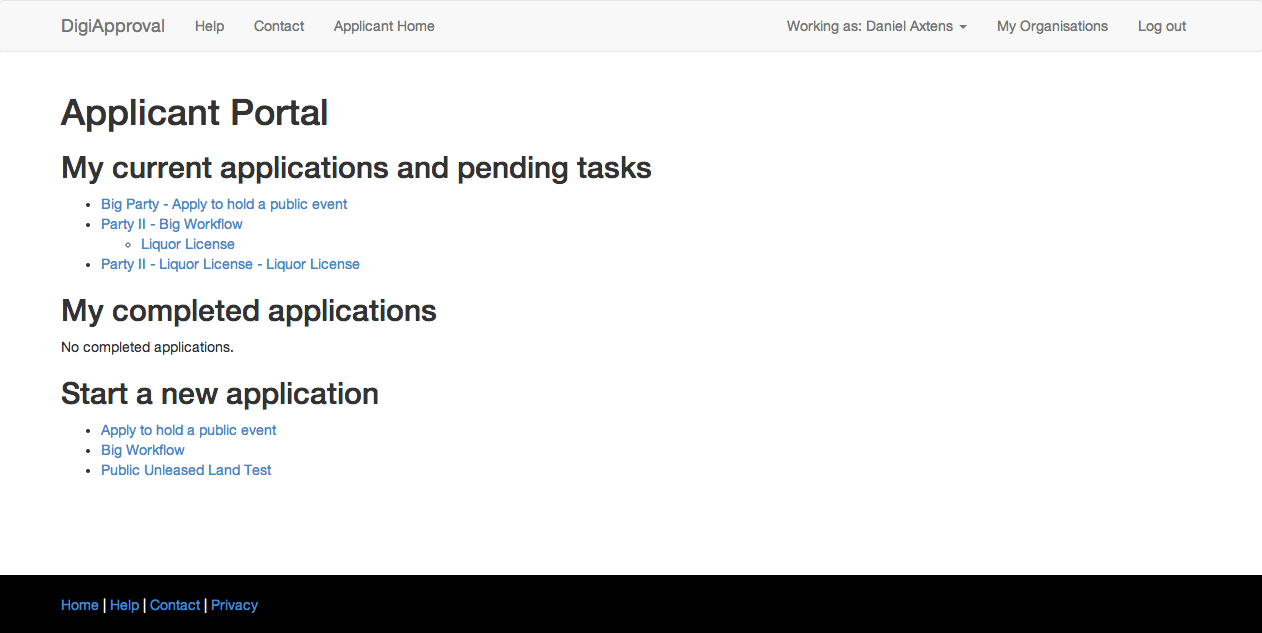
\includegraphics[width=0.9\textwidth]{customer-portal.png}
  \caption{The customer portal.}
  \label{fig:customer-portal}
\end{figure}

\subsubsection{Directorate experience}

\paragraph{Approver}

When an approver logs in, they can see at a glance (Figure~\ref{fig:approver-portal}):

\begin{itemize}

\item
  The applications for which they are responsible.
\item
  The status of those applications:

  \begin{itemize}
  
  \item
    Are they waiting on the applicant?
  \item
    Are they waiting on another agency?
  \item
    Are they ``in my court''?
  \end{itemize}
\end{itemize}

\begin{figure}[h!]
  \centering
  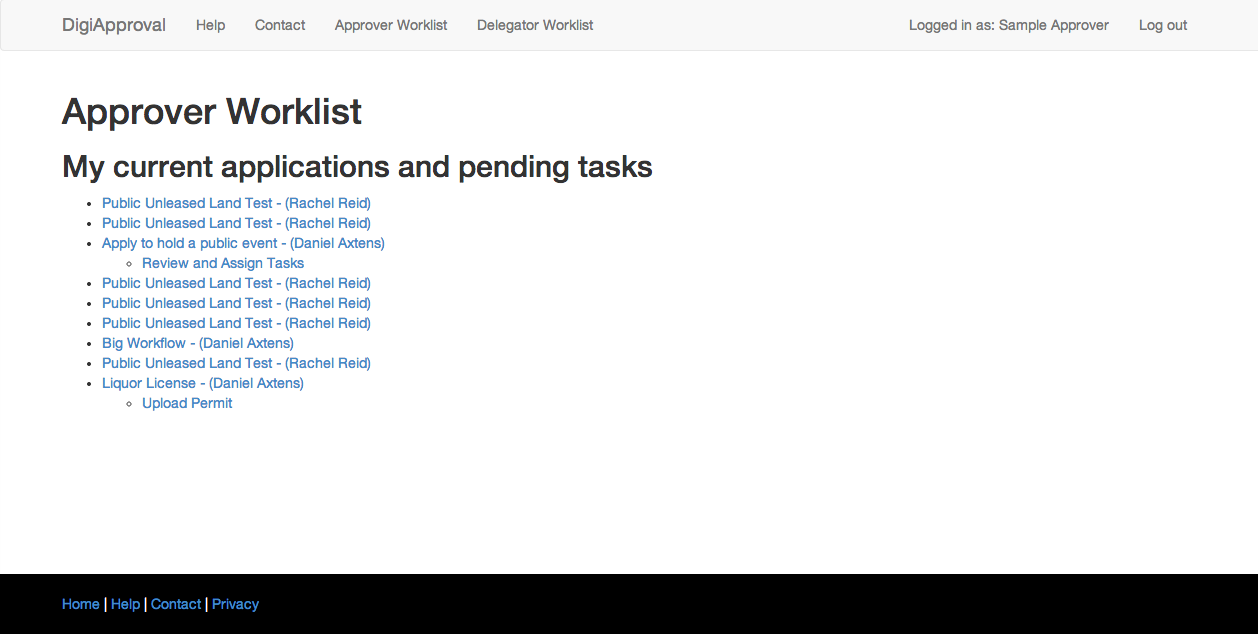
\includegraphics[width=0.9\textwidth]{approver-portal.png}
  \caption{The approver portal.}
  \label{fig:approver-portal}
\end{figure}

Approvers can then pull up an application (Figure~\ref{fig:approver-workflow}) for which they are
responsible and see in one place:

\begin{itemize}

\item
  The entire history of the application
\item
  All the communications that have been exchanged
\item
  Any steps necessary to progress it.
\end{itemize}

\begin{figure}[h!]
  \centering
  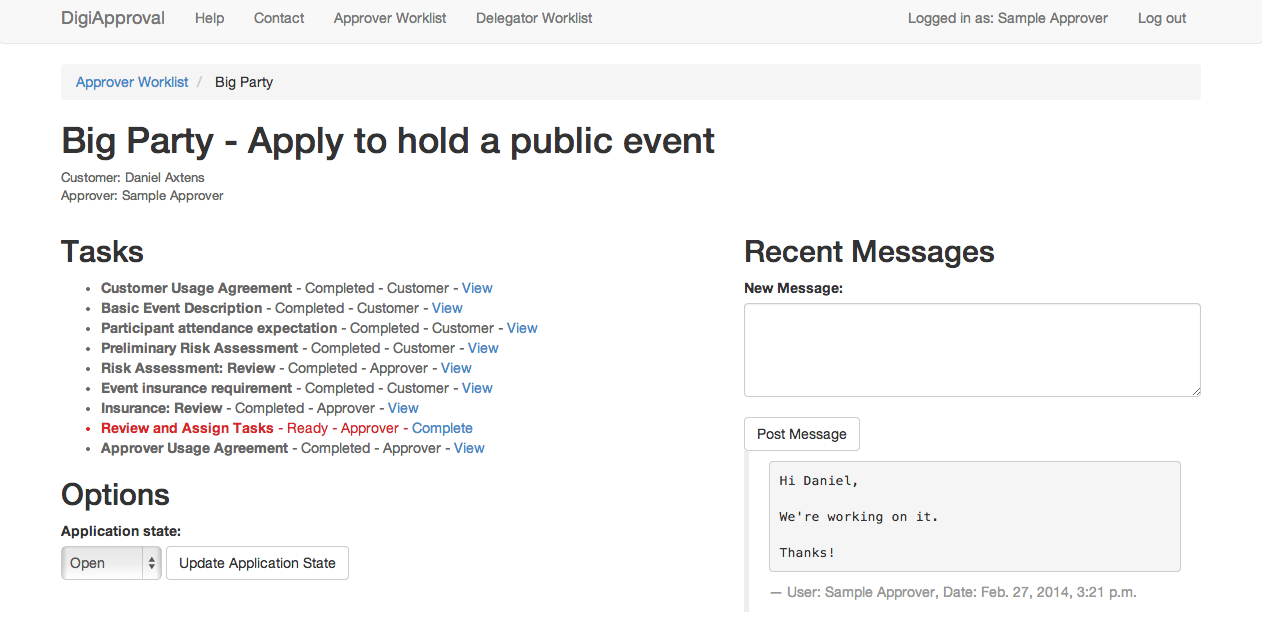
\includegraphics[width=0.9\textwidth]{internal-view.png}
  \caption{The workflow approval view.}
  \label{fig:approver-workflow}
\end{figure}

\paragraph{Delegators}

A delegator has a simple user interface to re-allocate in-progress
workflows if needed. (For example, if an approver is ill or leaves the
directorate.)

\subsubsection{Baked-in flexibility: point and click workflow design.}

Finally, administrators can build workflows from scratch using a
point-and-click editor (Figure~\ref{fig:workflow-editor}). All aspects of the workflow can be configured:
the tasks, their specifications, what information is provided to users,
who is responsible for them, task dependencies and so on.

\begin{figure}[h!]
  \centering
  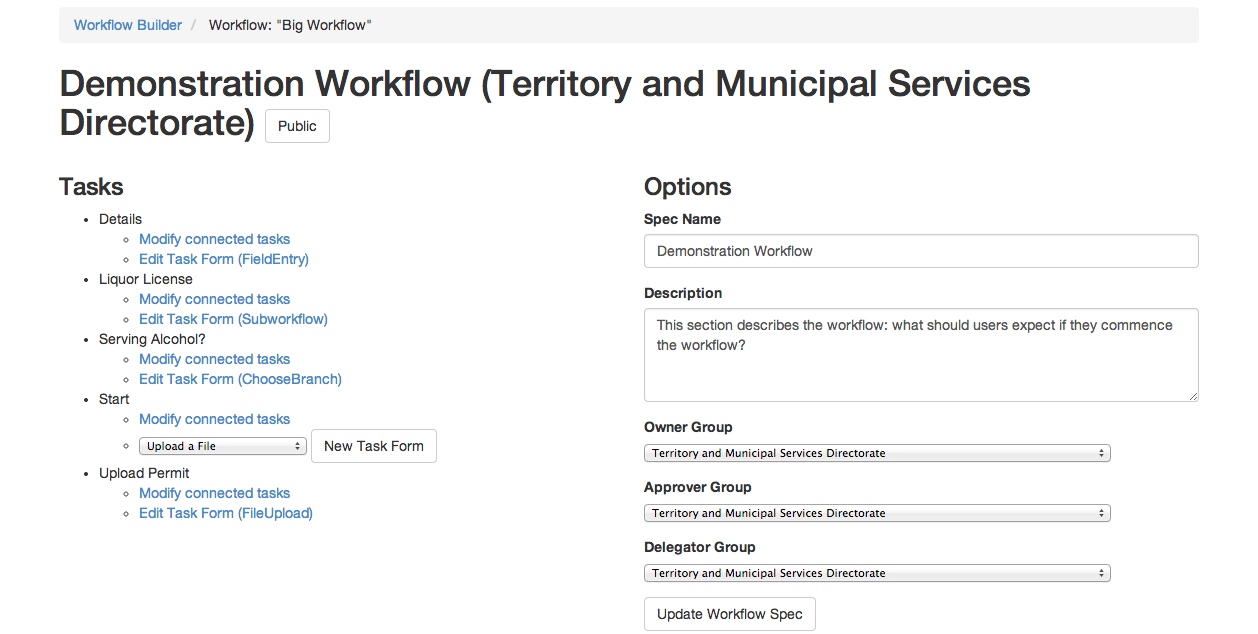
\includegraphics[width=0.9\textwidth]{workflow-editor.png}
  \caption{The workflow editor.}
  \label{fig:workflow-editor}
\end{figure}


Workflows are also automatically rendered as flowcharts (Figure~\ref{fig:workflow-flowchart}), 
for validation against with existing directorate procedures. (Obviously
\texttt{selection = 0} and \texttt{selection = 2} are not sufficient
descriptors. This is a known bug and would be fixed for a production
version.)

\begin{figure}[H]
  \centering
  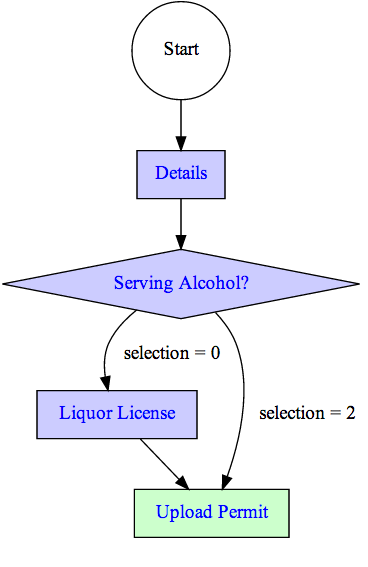
\includegraphics[width=0.5\textwidth]{workflow.png}
  \caption{A workflow flowchart.}
  \label{fig:workflow-flowchart}
\end{figure}

This ability to edit workflows online is a key feature which
distinguishes our solution from, for example,
\href{http://www.foxopen.net/}{FoxOpen}.

\subsection{The prototype: Tech Specs}

Our solution is a web application implemented with Python using the
Django web framework. It can be decomposed into a web layer, an
application layer, a set of asynchronous workers and a storage layer
(file store and database).

\begin{figure}[h!]
  \centering
  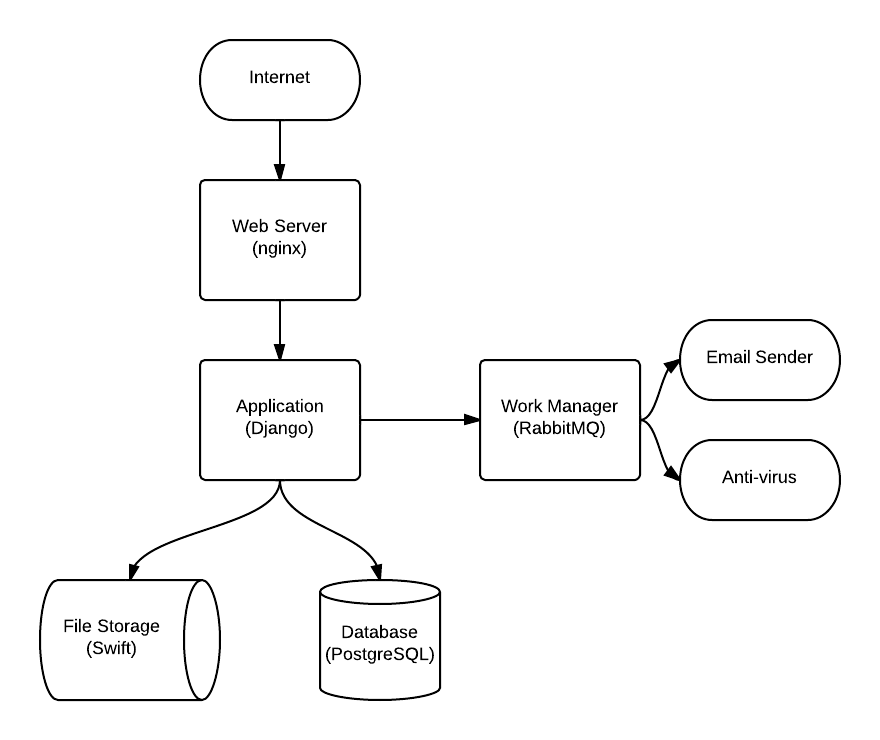
\includegraphics[width=0.8\textwidth]{./tech-overview.png}
  \caption{Technical stack of project.}
  \label{fig:solution-stack}
\end{figure}

Each of these layers is horizontally scalable.

Our system was built on:

\begin{itemize}

\item
  \textbf{Operating System}: \href{https://www.centos.org/}{CentOS 6.4} and \href{http://www.redhat.com/products/enterprise-linux/}{RHEL 6}

  \begin{itemize}
  
  \item
    Our stack should also port without issue to Solaris, as preferred by
    SSICT.
  \end{itemize}
\item
  \textbf{Provisioning}: \href{http://www.opscode.com/chef/}{Chef Solo},
  meeting the SSICT requirement for managed configuration over ad-hoc
  configuration.
\item
  \textbf{Web server}: \href{http://nginx.org/en}{nginx}.
\item
  \textbf{Application}: \href{http://django.org}{Django}

  \begin{itemize}
  
  \item
    A preference for using existing modules as opposed to developing our
    own functionality.
  \item
    The workflow engine is
    \href{https://github.com/knipknap/SpiffWorkflow}{SpiffWorkflow}.
  \end{itemize}
\item
  \textbf{Worker layer}: \href{http://rabbitmq.com}{RabbitMQ},
  interfaced through \href{http://www.celeryproject.org/}{Celery}.

  \begin{itemize}
  
  \item
    Virus scanning workers implemented in
    \href{http://www.clamav.net/lang/en/}{ClamAV}.
  \item
    Email workers send mail through \href{http://sendgrid.com/}{SendGrid}, using the SMTP interface
    for simple transition to SSICT infrastructure.
  \end{itemize}
\item
  \textbf{Database}: \href{http://postgresql.org}{PostgreSQL}.

  \begin{itemize}
  
  \item
    Transition to an Oracle database to meet SSICT requirements should
    be straightforward thanks to Django's database abstraction.
  \end{itemize}
\item
  \textbf{File storage}: \href{http://swift.openstack.org}{OpenStack
  Swift}.
\item
  \textbf{Front end}: \href{http://getbootstrap.com/}{Bootstrap} and
  \href{http://html5boilerplate.com/}{HTML5 boilerplate}

  \begin{itemize}
  
  \item
    Developed with an eye towards standards compliance, accessibility
    and extensibility.
  \end{itemize}
\end{itemize}

\subsubsection{The choice to use FOSS}

We chose to build our solution on an open source stack. Practically, we
had a number of reasons for choosing open source, including price, ease
of access and cross-platform compatibility. More fundamentally, open
source software has played a huge role in bringing technological
innovations to those who would otherwise not have had access to them,
and that's very much in line with how we saw the Digital Canberra
Challenge. As detailed in the next section, we were very happy with the
open source stack.

\subsubsection{In retrospect: how did our technology stack perform?}

We were very pleased with the performance of our technology stack.

\paragraph{The good}

\begin{itemize}

\item
  The stack performed exceptionally well at narrowing the functional
  areas we had to consider. So much was done for us that our actual
  application code comes in at less than five thousand SLOC (source
  lines of code) - an astonishingly low figure for what the system
  achieves.
\item
  By and large, the stack was reliable and high performance. We spent
  comparatively little time delving into the internals of the stack, and
  the majority of the time building on it. It was fit for purpose.
\end{itemize}

\paragraph{The bad}

\begin{itemize}

\item
  We initially used Amazon SES for email, however, it failed to send to
  ACT government, so we made the transition to SendGrid.
\item
  Chef proved incredibly difficult and time-consuming. We may have been
  better to pick a different configuration management system. However,
  it seems any system we could have picked would have involved a
  significant learning curve, and we certainly made a number of
  beginners mistakes.

  \begin{itemize}
  
  \item
    On the plus side, Chef made transition from CentOS (which we used
    for local testing) to RHEL 6 (which we used on AWS) reasonably
    painless.
  \end{itemize}
\item
  We found a number of open source components (most notably SpiffWorkflow) had
  one or more issues which required our intervention to fix. Using them
  still provided a significant increase in productivity vis-\`{a}-vis
  writing equivalent functionality from scratch, and furthermore by
  contributing the changes upstream we are able to pass of the
  requirement of on-going maintenance elsewhere.
\item
  Django performed well, although we found the standard Django template engine
  limiting -- in hindsight, we would have installed an alternative template engine.
\item
  OpenStack proved tricky to set up. We eventually settled on
  \href{http://devstack.org/}{DevStack}, which was decent choice, but
  suffered regressions a couple of times.
\item
  We attempted to use \href{http://www.vagrantup.com/}{Vagrant} to
  smooth out hardware and software differences. This worked well up
  until a point, but wasn't quite as perfect as we had hoped. (See Other
  Remarks below.)
\end{itemize}

\subsection{How does this solution contribute to making Canberra a
digital city}

This solution ties in with the
\emph{\href{http://www.cmd.act.gov.au/policystrategic/digitalcanberra/actionplan}{Digital
Canberra Action Plan}} and
\emph{\href{http://www.cmd.act.gov.au/__data/assets/pdf_file/0011/247826/The_Strategic_Plan_for_ICT_2011-15.pdf}{The
Strategic Plan for ICT 2011-2015}}, which are whole-of-government
initiatives.

\begin{framed}
\begin{quote}
The Digital Canberra Action Plan is the roadmap of how we are going to:

\begin{itemize}

\item
  accelerate business engagement with the digital economy and help
  businesses access new customers and markets;
\item
  promote Canberra as a modern, dynamic, digital city;
\item
  use technology to be a more open government and to give citizens
  greater choice in how and when they use services; and
\item
  be more innovative in how we engage with the community and local small
  business.
\end{itemize}

(\href{http://www.cmd.act.gov.au/policystrategic/digitalcanberra}{Digital
Canberra website})
\end{quote}
\end{framed}

DigiApproval strongly complements the objectives of the Digital Canberra
Action Plan. In particular:

\begin{itemize}

\item
  by providing better visibility into permit applications, DigiApproval
  creates a more open government;
\item
  as an online service, it provides citizens greater choice:
  applications can be completed in stages, in different places;
\item
  having been designed with community groups in mind, it provides an
  innovative and improved experience for community groups and small
  businesses; and
\item
  its overall effect is to bring a modern, dynamic, digital approach to
  the process of applying for permits.
\end{itemize}

Furthermore, the DigiApproval system is aligned with the the goals and
governing principles of
\href{http://www.cmd.act.gov.au/__data/assets/pdf_file/0011/247826/The_Strategic_Plan_for_ICT_2011-15.pdf}{The
Strategic Plan for ICT 2011-2015}. The Strategic Plan identifies 5 key
goals for ICT within the ACT government:

\begin{quote}
\begin{enumerate}

\item
  Make living in Canberra easier by developing, with the community, an
  integrated, comprehensive and affordable range of readily accessible
  online services.
\item
  Improve return on investment on public expenditure on ICT through
  implementing and sharing higher quality, more resilient systems.
\item
  Use ICT to promote Open Government and online community engagement.
\item
  Contribute to the achievement of its environmental targets by
  improving the energy efficiency of its ICT infrastructure and
  promoting the use of ICT to assist other sustainability initiatives.
\item
  Develop its workforce and partnerships to provide the future capacity
  and skills to implement its ICT programs and strategies.
\end{enumerate}
\end{quote}

In particular, the system targets Goal 1, as part of an ``integrated,
comprehensive and affordable range of readily accessible online
services.'' In particular, it ``will use ICT to provide simpler
citizen-centric services, integrated across Directorates'' (page 8).

DigiApproval can contribute to the goals of being:

\begin{itemize}

\item
  \textbf{integrated}, including being \textbf{integrated across
  Directorates} - the system is designed to integrate application
  processes across directorates by defining a shared vocabulary (the
  semantic tags described above) and a well-understood data flow. In
  this way, the system provides both sufficient flexibility and
  integration.
\item
  \textbf{comprehensive}, as it can model arbitrary workflows - it would
  be suitable for any permit application, or even other government tasks
  that can be modelled as workflows.
\item
  \textbf{affordable}, as it increases efficiency - reduced paper-work
  and speedier interaction with the client means that files can be
  processed and closed out faster.
\item
  \textbf{readily accessible}, as it requires no specialised software
  either on the user or Directorate end; just a web browser.
\item
  \textbf{simpler} for both citizens and directorates - by doing
  applications piece-wise and with an integrated communications
  register, it enables questions to be asked during the process, and
  enables feedback to be given on an on-going basis through the
  application process, rather than in one big hit.
\item
  \textbf{citizen-centric}, as it was driven by citizen-lead design via
  the Digital Canberra Challenge. It addresses citizen pain points by
  incorporating a single point of contact, and visibility into the
  process.
\end{itemize}

Furthermore, the solution is in line with a number of other goals:

\begin{itemize}

\item
  Goal 2:

  \begin{itemize}
  
  \item
    The DigiApproval system has been built in line with the Shared
    Services ICT requirements, so it can be implemented more cheaply and
    with less friction, \emph{improving ROI}.
  \item
    The DigiApproval system is designed to be a \emph{shared},
    cross-Directorate system.
  \end{itemize}
\item
  Goal 4: Implementing the DigiApproval system will significantly
  decrease the amount of paper used in the approval process.
\item
  Goal 5: By virtue of the Digital Canberra Challenge process, the
  project is being implemented as a public-private partnership,
  increasing the capacity within Canberra.
\end{itemize}

Furthermore, the project can be implemented in line with the Governing
Principles laid out on page 7 of the Strategic Plan.

The principles are:

\begin{quote}
\begin{itemize}

\item
  investment should support Government policy and service delivery
  priorities.
\item
  should be of a professional quality, lifecycle managed and
  supportable.
\item
  investment should create improved performance, greater efficiency and/
  or better community services.
\item
  should be shared wherever possible across Government.
\item
  \ldots{}
\item
  investment must have measurable outcomes.
\end{itemize}
\end{quote}

Investment in this system would be in line with those principles:

\begin{itemize}

\item
  It supports service delivery by assisting directorates to meet their
  legislative requirements for service delivery.
\item
  It is of professional quality, and supportable - see the
  Sustainability section below.
\item
  It creates improved performance, greater efficiency and better
  community services, as outlined.
\item
  It can be readily shared across government, and used for both
  citizen-facing and internal workflows.
\item
  The outcome of an investment into the system can be measured in terms
  of reduction in directorate time and cost per application.
\end{itemize}

\newpage
\section{Production system}

The system has been designed with production in mind.

\subsection{Sustainability}

Our system is sustainable from a number of different angles. In
particular, we have focused on \textbf{sustaining the capacity of the
system to function as desired}, in particular by reducing dependence on
the DigiACTive team.

\subsubsection{Implementation of the system within directorates}

Because of the point-and-click workflow editor, the system can be
implemented across directorates without needing the DigiACTive team's
intervention.

\subsubsection{Ongoing use of the system within directorates}

The system is designed to be tolerant to changes in staffing within a
directorate.

\begin{itemize}

\item The delegator/approver system provides a simple approach to
  re-allocating work as staff arrangements change. It provides direct
  visibility into the workload of approvers, and allows it to be
  adjusted as needed.
\item
  The system is also designed to be sustainable in the sense that it's
  integrity is not threatened when staff members leave. Each staff
  member has an individual user account, which can be easily deactivated
  when they leave.
\end{itemize}

The system is also designed to be tolerant to changes in business
processes: the point-and-click editor enable these changes to be
reflected in the workflow models ``in house'', without requiring
DigiACTive to write any code.

\subsubsection{Ongoing use within community organisations}

A major complaint that drove the challenge was the need to reduce the
duplicated effort that occurs when a community group runs similar events
repeatedly. The permanent archival of past applications means previous
information is always available.

Furthermore, the differentiated registration for community groups is
designed to maintain their capacity in the face of changing membership.

\begin{itemize}

\item
  It allows group membership to change without losing any information:
  when a group member leaves the group, they do not take any information
  with them. All applications made on behalf of the community group stay
  on archive and are accessible to members of the group.
\item
  It maintains the integrity of the community group's application
  process: once a member leaves or is removed from the group, they can
  no longer take actions on behalf of the group.
\end{itemize}

\subsubsection{Sustainable software stack and toolset}

The system has been designed and built such that if the DigiACTive team
were hit by a bus, it would be possible to hire replacement staff that
could quickly come up to speed on the system.

To that end:

\begin{itemize}

\item
  The system is built on widely used, open source software, as detailed
  in the technical specs.
\item
  Our implementation has consistently preferred to integrate prebuilt
  software packages rather than reinvent the wheel. This means:

  \begin{itemize}
  
  \item
    Our code conforms to the conventions required by those packages.
  \item
    Our code base is small (less than five thousand SLOC) -- only
    implementing those things not implemented in other software.
  \end{itemize}
\item
  We have an automated unit test suite.
\end{itemize}

\paragraph{Contributing to the open-source ecosystem}

As we have built on open-source software, we have occasionally found
that we need to fix a particular bug or extend a particular feature in
the software we are using. We have consistently sought to contribute
these changes back. This has a number of benefits:

\begin{itemize}

\item
  It contributes to the open-source eco-system, which we in turn benefit
  from.
\item
  It shifts the responsibility for maintaining our changes away from us
  and back to the original maintainer of the package, reducing our
  ongoing workload.
\end{itemize}

\subsubsection{Sustainable software}

The system is designed to remain viable in the face of changing
requirements.

\begin{itemize}

\item
  The system has been built in a generic way, such that it can be
  extended without breaking existing functionality.
\item
  The underlying workflow engine supports a number of features that have
  not been exposed in the user interface, so a number of feature
  requests are as simple as writing a front end.
\item
  A lot of thought and careful planning has gone into the data model and
  interconnections -- this gives us confidence that we can hook up the
  system to other systems such as a payment system without undue
  difficulty.
\end{itemize}

\subsection{Scalability}

The system is designed to be scalable from the ground up.

\begin{itemize}

\item
  Technically, the system can easily scale up to arbitrary user load.
  The system is ``loosely coupled'': everything easily disaggregates and
  multiplies.
\item
  In terms of usage, the system can scale up from being used by a small
  test group to universal usage without issue, so long as the paper and
  online workflows are kept in sync.
\item
  The system can scale across directorates:

  \begin{itemize}
  
  \item
    The authentication system allows multiple directorates to use shared
    system, without stepping on each others' toes.
  \item
    Furthermore, with subworkflows - the ability to integrate workflows
    into other workflows - scaling up to more directorates and areas
    will enhance the system rather than degrade it.
  \end{itemize}
\end{itemize}

\subsection{Integration}

The system is designed to seamlessly integrate with existing directorate
processes.

\begin{itemize}

\item
  The system has been built with the intention of allowing powerful
  reporting capabilities. This would be implemented in a production
  system.
\item
  The system models existing workflows rather than requiring existing
  workflows to be replaced, thus reducing the friction for integration.
\item
  The system architecture allows easy interfacing with external systems, such as existing document management systems or other web applications.
\end{itemize}

\subsection{The bottom line}

As the DigiApproval system is currently at proof of concept stage,
preparing it for public deployment will require a further investment of
time and money.

DigiACTive estimates that a further 500-600 person hours of software
development time would be required to make the software production
ready, in addition to the skills of a graphics designer and a user
experience designer. If this process was started immediately, the
software could be ready for public deployment as early as July 2014.


\newpage
\section{Concluding remarks}

We had an overwhelmingly positive experience of the competition. In the
course of a few months, we have gone from a group of friends at the
Australian National University to a proprietary limited company with a
proof of concept system that has commercial potential. We have worked
productively with NICTA and with TAMS to deliver on the agreed
objectives.

\textbf{From the point of view of DigiACTive, the Digital Canberra
Challenge has been hugely successful.} The project was excellently
managed by the eGov Cluster, and TAMS has been incredibly helpful
throughout the process.

\subsection{Suggestions for future rounds}

In order to proceed in the bake-off, we required a formal legal
structure. We consulted a lawyer, and opted to form a proprietary
limited company. We were also required to acquire insurance as part of
the bake-off agreement.

We were fortunate to have team members with experience as sole traders
and in forming incorporated associations. Nonetheless, we found the
administrative process of forming a company, getting the necessary
insurance, and sorting out the necessary legal documents to be, on the
one hand, immensely educational, and on the other hand, incredibly
time-consuming, expensive and frustrating. It consumed the bulk of our
time for the first several weeks of the competition, and consumed well
over half of our total project budget.

If we had an pre-existing company, we could have redirected our time and
money towards a number of different things. For example, if we had been
less pushed for time and money, we would have brought a graphic designer
and a user experience specialist on board.

On the plus side, being pushed to have a formal legal structure has set
us up well to continue the project into the future. On the down side, if
we choose not to proceed, we have to wrap up the company, sort out its
tax affairs, and so on: we're left holding a time-consuming liability.

We therefore have a number of suggestions for future competitions:

\begin{itemize}
\item
  We would have benefited from some sort of information session or
  information pack outlining matters such as:
\begin{itemize}
\item 
  different business structures: e.g.~company vs partnership
\item
  how to go about forming one: applying directly through ASIC v applying
  through e.g.~MYOB CompanyDocs
\item
  the legal agreements needed to protect us, e.g.~a Shareholders'
  Agreement
\item
  establishing appropriate accounting systems
\item
  the various different types of insurance we would require
\item
  how we would go about expanding or winding up a company after the
  competition
\end{itemize}
\item
  SMEs have a distinct advantage compared to other entrants because of
  their existing company structure: they don't need to spend any of
  their budget on forming a company. It may be worth considering a rebalancing
  of this advantage.
\item
  The insurance requirement could be re-evaluated. We were required to
  hold professional indemnity insurance to guard against direct loss to
  the government. However it is hard to see how the proof of concept
  could actually cause the government financial loss, given that it was
  not hosted on government servers, did not process payments, and did
  not process actual user data.
\end{itemize}

\newpage
\section{Other remarks}

We have one suggestion for future teams, and two specific suggestions
for teams coming from non-commercial, academic or otherwise low-budget
environments.

\subsection{General}

A major thing we had to adapt to is the very different way of thinking
in the government space versus the innovation/start-up space.

The process we had was very linear: gather requirements, develop a
design document, build the system. Approval and sign-off was required at
each stage. This is in sharp contrast to the way we were used to
operating: build a prototype, present it, see how people actually use it
and what they want changed, fix the prototype in response, get more
feedback and so on.

Absent the more formal process, we would have attempted to build a
minimum viable product by iteration rather than through explicit design.
However, the formal process actually worked out better than we were
expecting, because feedback was less interactive than we were used to.
We didn't, for example, have the opportunity to just hover over peoples'
shoulders as they attempted to use the demonstration systems. Feedback
took longer to get and was a very different sort of feedback to what we
would have needed for the minimum viable product/iteration model to be
effective.

From time to time we found the more formal process slow, restrictive and
frustrating. We would advise future teams to stick at it and make sure
it is done well -- we found the things we hadn't designed as thoroughly
to be the ones we struggled with more.

\subsection{For those from non-commercial/academic environments in
particular}

\begin{itemize}
\item
  One of our biggest and most surprising time-sinks arose from the
  different hardware we had. Two of our members had Macs, and one had
  a PC running Linux. Despite our best efforts to
  make the development environment consistent through the use of
  Vagrant, we found a lot of time still disappeared in the differences
  Vagrant couldn't quite smooth out. \textbf{It's worth getting
  identical systems somehow:} either by buying identical hardware, or by
  doing all your development in the cloud from the start.
\item
  It's very tempting to not name a leader, especially as a group of
  friends. However, \emph{there are no leaderless groups:} someone will
  end up leading; sometimes different people at different points, but
  someone must take the lead for things to get done. We would have
  benefitted from picking a leader at the start, and would advise future
  groups to do so.
\end{itemize}
\end{document}
